\documentclass{beamer}
\usetheme{Madrid}
\usepackage{pgfplots}
\pgfplotsset{compat=1.15}
\usepackage{mathrsfs}
\usetikzlibrary{arrows}
\usepackage[utf8]{inputenc}
\usepackage{xcolor}
\usepackage{hyperref}
\usepackage{fancyvrb}
\usepackage{comment}
\usepackage{listings}
\usepackage{color}
\definecolor{munsell}{rgb}{0.0, 0.5, 0.69}
\definecolor{dkgreen}{rgb}{0,0.6,0}
\definecolor{gray}{rgb}{0.5,0.5,0.5}
\definecolor{mauve}{rgb}{0.58,0,0.82}
\definecolor{minas}{RGB}{0.244, 0.172, 0.36}
\definecolor{PUJ}{RGB}{44, 86, 151}
\definecolor{PUJ2}{RGB}{43, 93, 156}
\definecolor{PUJ3}{RGB}{20, 52, 107}
\definecolor{cyandk}{rgb}{0.0, 0.72, 0.92}
\setbeamerfont{frametitle}{size=\LARGE ,series=\bfseries}
\setbeamercolor{frametitle}{fg=PUJ2, bg=white} %% title of the beamer
\setbeamercolor{titlelike}
{parent=structure,bg=PUJ2}
\setbeamercolor{title}{fg=white, bg=PUJ3} 
%\setbeamercolor{navigation symbols}{fg=white, bg=white}
\setbeamercolor*{palette primary}{use=structure,fg=black,bg=yellow}
\setbeamercolor*{palette secondary}{use=structure,fg=white,bg=PUJ3}
\setbeamercolor*{palette tertiary}{use=structure,fg=white,bg=PUJ3}

\setbeamercolor{block title}{bg=PUJ3,fg=white}


%% code information
\lstset{frame=tb,
  language=Python,
  aboveskip=3mm,
  belowskip=3mm,
  showstringspaces=false,
  columns=flexible,
  basicstyle={\small\ttfamily},
  numbers=none,
  classoffset=1,
  morekeywords={True,False}, keywordstyle=\color{munsell}, 
  classoffset=0, 
  keywordstyle=\color{blue},  
  commentstyle=\color{dkgreen},
  stringstyle=\color{PUJ3},
  numberstyle=\tiny\color{gray},
  breaklines=true,
  breakatwhitespace=true,
  tabsize=4,
}

%% You can change default language in the middle of document with \lstset{language=Java}.


%% PUT or Remove the logo in a slide.


%% Information topic

\institute{Javeriana}
\date{2020}

\title[Pontificia Universidad Javeriana] %optional
{Monty Hall simulation}
\subtitle{Using python.}

\author[Iván Andrés Trujillo Abella] 
{Iván Andrés Trujilllo Abella}

\institute[] 
{
  Facultad de Ingenieria\\
  Pontificia Universidad Javeriana
  \and
  
\textbf{ trujilloiv@javeriana.edu.co}
}

\date[MINTA] % (optional)

\newif\ifplacelogo % create a new conditional
\placelogotrue % set it to true
%\logo{\ifplacelogo\color{red}\rule{.5cm}{.5cm}\fi}
\logo{\ifplacelogo 
\includegraphics[height= 2.0cm]{pujshield.eps}\fi}



\begin{document}

\frame{\titlepage}



\begin{frame}{Monty Hall simulation}
\begin{block}

This problem is so not intuitive that generated controversy in the academic community. 
\end{block}

There are three closed doors,  and you must select one to win  a car,  behind the doors, there is a car, and behind the other two there are goats. After select the door, another door with a goat it is showed to you, then you can change your first election,  the main problem is if you must remain in the selected door or change?

Notice that the initial probability of win the car is the 1/3.
\end{frame}



\begin{frame}{Monty Hall simulation}{}
\begin{figure}[htbp]
\centerline{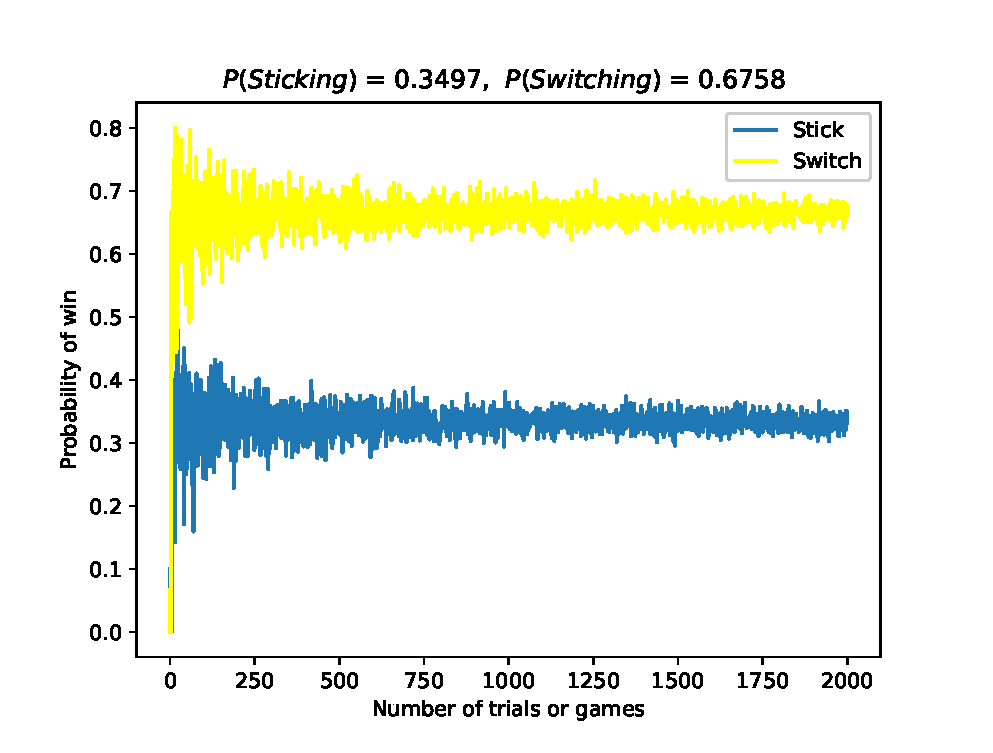
\includegraphics[scale=0.66]{./graphs/Monty.eps}}
\end{figure}
\end{frame}





\begin{frame}[fragile]{Monty Hall problem}{Python code}
\begin{lstlisting}
def monty_game():
  doors=[1,2,3]
  doors_variable = doors.copy()
  winner = random.randint(1,3)
  select_one = random.randint(1,3)
  values = [winner,select_one]
  switch = list( set(doors) - set(values))
  select_two = random.randint(switch[0], switch[-1])
  s1,s2 = 0,0
  if winner == select_one:
    s1 += 1
  else:
    s2 +=1
  return [s1,s2]
\end{lstlisting}
\end{frame}


\begin{frame}[fragile]{Monty Hall problem}{Python code}
\begin{lstlisting}
trials=2000
s1_=[]
s2_=[]
for n in range(1,trials):
  prob_s1 = sum([monty_game()[0] for _ in range(1,n)])/n
  s1_.append(prob_s1)
  prob_s2 = sum([monty_game()[1] for _ in range(1,n)])/n
  s2_.append(prob_s2)
plt.plot(np.arange(1,trials),s1_, label='Stick')
plt.plot(np.arange(1,trials),s2_, label='Switch',color='yellow')
plt.title('$P(switching)$ = {:.4},  $P(sticking)$ = {:.4} '.format(prob_s1,prob_s2))
\end{lstlisting}
\end{frame}



\begin{frame}{Monty Hall}{Bayesian solution}
The event $D_{i}$ the $i$ winner door and  $M_{j}$ monty open $j$ door, for $i,j=1,2,3$.

\begin{equation}
P(D_{i} \mid M_{j}) = \frac{P(M_{j} \mid D_{i})P(D_{i})}{P(M_{j})}
\end{equation}

you select the first door  and monty the second, therefore the question  is $P(D_{3} \mid M_{2})$.
Notice that $ P(M_{2}) = \sum_{i=1}^{3} P(M_{2} \mid D_{i}) $.  
given the rules of game, 
$P(M_{2} \mid D_{2}) = 0$, and 
$P(M_{2} \mid D_{3}) = 1$, if monty could select random in two choices $P(M_{2} \mid C_{1})=1/2$ and finally, switch strategy have a probability of 2/3.
\end{frame}

\end{document}